% vim: set spl=en:
\documentclass[smaller,t]{beamer}
\usepackage[utf8]{inputenc}
\usetheme{westlife}

\def\code#1{\structure{\texttt{#1}}}
\def\nadpis#1{\par\medskip\textbf{#1}}

\begin{document}
\makeatletter

\title{Virtualized Web Portals in EGI \\[\smallskipamount] Federated Cloud}
\date{MUSTweek, Brno, March 5--10}
\author[A. Křenek et al.]{Aleš Křenek, Radim Peša, Tomáš Raček, Vlastimil Holer, Daniel Kouřil, Ĺubomír Ontkoc}
\begin{frame}
\maketitle
\end{frame}

\begin{frame}{Why to virtualize web portals}

\end{frame}

\begin{frame}{Available sofware solutions}

\end{frame}

\begin{frame}{Typical portal architecture}

\end{frame}

\begin{frame}{Deployment bottom-up}

\end{frame}

\begin{frame}{Deployment top-down}

\end{frame}

\begin{frame}{Tutorial overview}
\begin{itemize}
\item Understand the homework 
\begin{itemize}
\item obtain X.509 certificate and register it with VO
\item setup client environment -- software, CA certificates, VO servers, \dots (docker container)
\item check that occi works (interact with FedCloud site)
\item do the magic deployment out of blackbox 
\item \alert{let's understand it}
\end{itemize}
\item Deploy web application 
\begin{itemize}
\item start with non-claudified (but cleaned up) application code
\item \alert{extend Tosca description}
\item \alert{provide specific configuration scripts}
\end{itemize}
\end{itemize}
\end{frame}

\begin{frame}{Tutorial overview}
\begin{itemize}
\item Add worker node
\begin{itemize}
\item start with working web front end
\item pick another example -- Torque server + worker node
\item \alert{merge two Tosca specifications}
\item \alert{configure multi-node interaction}
\end{itemize}
\item Real-world user authentication
\begin{itemize}
\item start with working application with fake user
\item \alert{set up service provider and connect with IdP proxy}
\end{itemize}
\end{itemize}
\end{frame}


\begin{frame}{The application -- SAXS ensemble fit}
\begin{center}
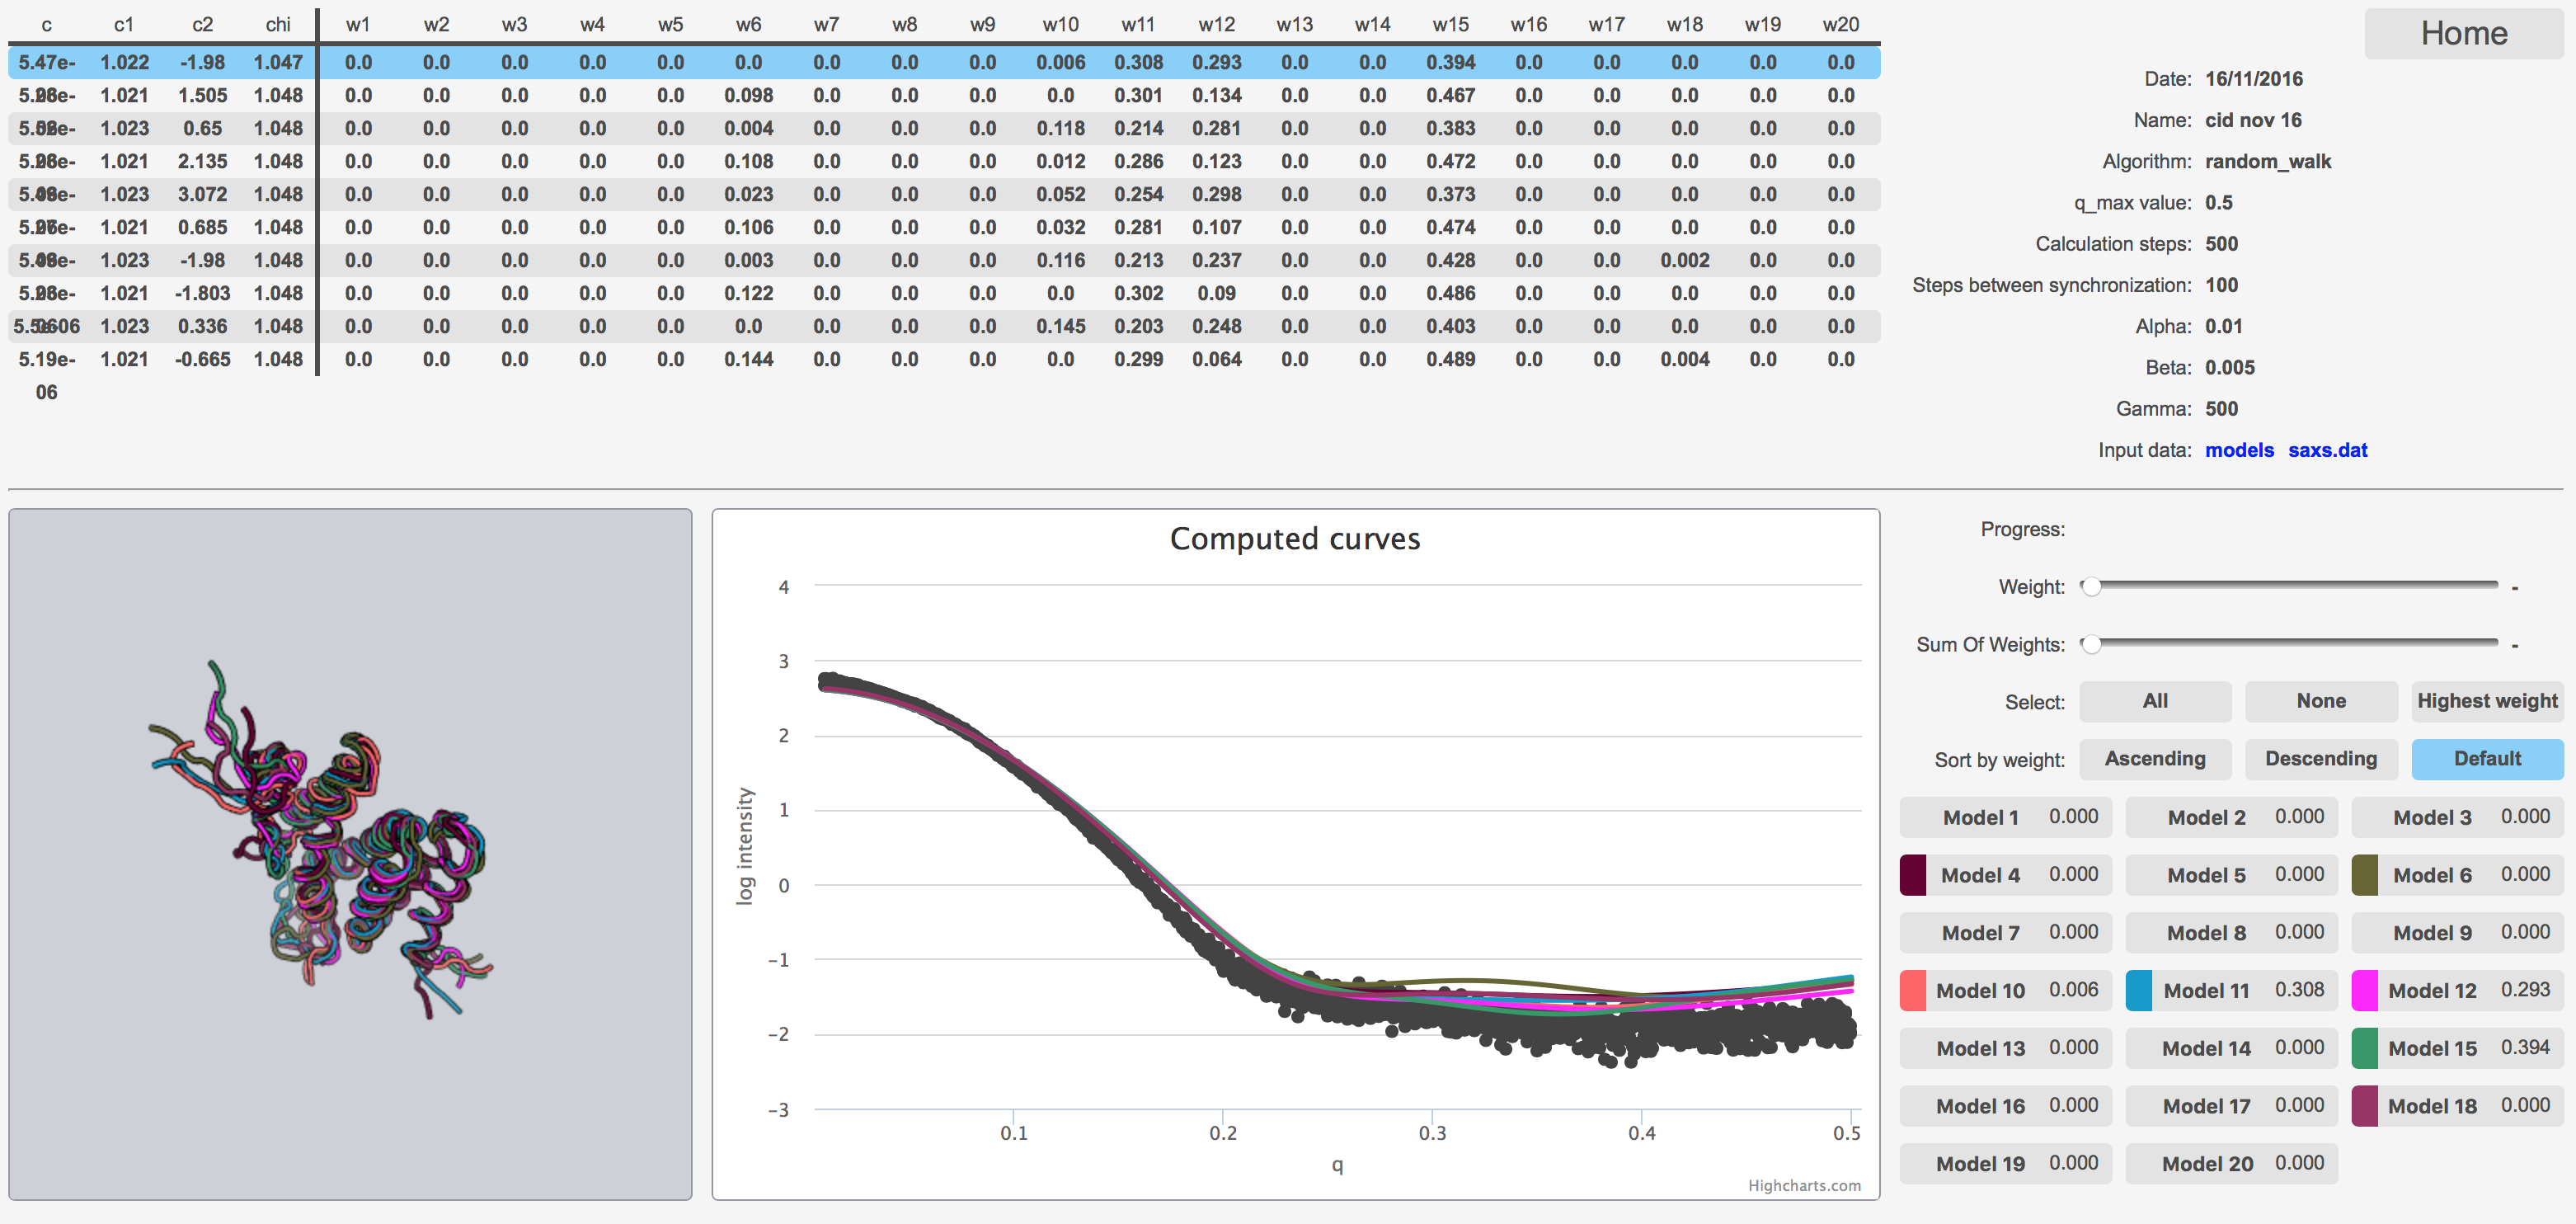
\includegraphics[width=.95\hsize]{saxs_cid}
\end{center}
\end{frame}

\begin{frame}{Bricks to be used}
\begin{itemize}
\item Apache server
\begin{itemize}
\item single node deployment
\item set up a VM using bare OS image (CentOS 7) using OCCI
\item use Puppet to configure Apache web server with ``Hello, world!'' CGI script
\item we will use it ``as is'', not touching internals (deployment scripts, Puppet recipes, \dots)
\end{itemize}

\item Torque server + worker node
\begin{itemize}
\item two node deployment
\item standalone, independent on the Apache one
\item complex Puppet configuration again
\end{itemize}
\end{itemize}
\end{frame}

\begin{frame}{Don't panic!}
\begin{itemize}
\item It is rather complex work, we know
\item Many things can go wrong
\item We will do the work step by step
\item Use local git commits to preserve work
\item Emergency checkpoints
\begin{itemize}
\item working implementations of the major steps
\item you can pick them if you get really lost 
\end{itemize}
\end{itemize}
\end{frame}



\begin{frame}{Understand the homework}
\begin{itemize}
\item In your Docker container (\code{radimpesa/mustweek2017})
\begin{itemize}
\item initialize cloudify: \code{\# source \$HOME/cfy/bin/activate}
\item do a fresh clone of \texttt{git@github.com:ICS-MU/westlife-mustweek2017.git}
\item look into \texttt{apache/} folder
\end{itemize}

\item M4 preprocessing to distinguish local vs.\ CFM deployment 
\begin{itemize}
\item ignore today, just don't edit the generated \texttt{.yaml} files
\end{itemize}
\item browse the \texttt{.yaml} files 
\begin{itemize}
\item blueprint and inputs in the main 
\end{itemize}
\item deploy: \code{\# make cfy-deploy}
\begin{itemize}
\item check the result, see \code{\# cfy local outputs}
\end{itemize}
\item cleanup: \code{\# make cfy-undeploy}
\end{itemize}

\end{frame}


\end{document}
